%% main_report37.tex
%% SAMBP TR-37/2026: Monte Carlo Reliability Assessment of IBR Protection Scheme
%%
%% pdflatex main_report37.tex

\documentclass[11pt,a4paper]{article}

\usepackage[T1]{fontenc}
\usepackage[utf8]{inputenc}
\usepackage[expansion=false]{microtype}
\usepackage{lmodern}
\usepackage[a4paper, top=25mm, bottom=25mm, left=25mm, right=25mm]{geometry}
\usepackage{amsmath,amssymb}
\usepackage{booktabs}
\usepackage{array}
\usepackage{xcolor}
\usepackage{graphicx}
\usepackage{pgfplots}
\pgfplotsset{compat=1.18}
\usepackage{tikz}
\usetikzlibrary{arrows.meta,shapes.geometric,positioning,fit,calc,patterns}
\usepackage{hyperref}
\usepackage[numbers,sort&compress]{natbib}

\definecolor{sambpblue}{RGB}{0,70,140}

\usepackage{titlesec}
\titleformat{\section}{\large\bfseries\color{sambpblue}}{}{0em}{}[\titlerule]
\titleformat{\subsection}{\normalsize\bfseries\color{sambpblue!80}}{}{0em}{}

\usepackage{fancyhdr}
\pagestyle{fancy}
\fancyhf{}
\rhead{\small\color{gray} SAMBP TR-37/2026}
\lhead{\small\color{gray} Monte Carlo Reliability Assessment}
\cfoot{\small\thepage}

\begin{document}

\begin{center}
  {\LARGE\bfseries\color{sambpblue} SAMBP Technical Report TR-37/2026}\\[6pt]
  {\large Monte Carlo Reliability Assessment\\
    of the IBR Distance Protection Scheme}\\[10pt]
  {\normalsize PhD Thesis Supporting Report \quad|\quad 2026}
\end{center}

\vspace{2pt}\hrule\vspace{8pt}

\begin{abstract}
\noindent
This report provides a Monte Carlo reliability assessment of the complete IBR
line protection scheme developed in TR-29--TR-36.  4000 fault scenarios are
sampled from physically motivated distributions ($k_\mathrm{ibr}\sim U[0.04,0.50]$,
$\alpha\sim U[0,1.05]$, fault type weighted by CIGRE statistics, arc resistance
exponential with mean 4\,m$\Omega$).  The scheme achieves overall dependability
$P_\mathrm{dep}=99.61\%$; all 15 missed faults have $k_\mathrm{ibr}<0.06$
(below the 87L current threshold) and are structurally unprotectable by any relay
element.  Fast clearance (within $T_\mathrm{mem}=100$\,ms) is 100\% of all
cleared faults, with mean clearance time 20.4\,ms.  Regions~B, C, and~D
achieve $P_\mathrm{dep}=1.000$; Region~A reaches 97.09\% (the residual 2.91\%
are $k<0.06$ structural misses).  A four-scenario IBR-penetration sensitivity
study confirms $P_\mathrm{dep}=1.000$ for all scenarios with $k_\mathrm{ibr}\geq0.06$.
The auto-reclosing chain (TR-36) clears 100\% of permanent-fault reclose
scenarios via 87L (memory-independent).
\end{abstract}

\vspace{4pt}\hrule\vspace{10pt}

% ─────────────────────────────────────────────────────────────────────────────
\section{Methodology}
\label{sec:method}

\subsection{Sampling distributions}

Fault parameters are drawn independently at each trial ($N=4000$, \texttt{seed=42},
consistent with TR-08~\cite{SAMBP_TR08}):

\begin{center}
\begin{tabular}{@{}lll@{}}
\toprule
Parameter & Distribution & Notes\\
\midrule
$k_\mathrm{ibr}$ & $U[0.04,\,0.50]$ & Covers near-zero to strong IBR contribution\\
$\alpha$ & $U[0.00,\,1.05]$ & $\alpha>1.0$ classifies as external/OOB fault\\
Fault type & Weighted categorical & 3PH: 5\%, SLG: 70\%, LL: 20\%, LLG: 5\%\\
$R_\mathrm{arc}$ & $\mathrm{Exp}(\lambda=250)$, clipped $[0,0.025]$ & Mean 4\,m$\Omega$;
  metallic dominant\\
Fault nature & Bernoulli($p=0.85$) & 85\% transient, 15\% permanent (IEEE)\\
\bottomrule
\end{tabular}
\end{center}

\subsection{Protection scheme model}

Each trial evaluates the five-element scheme from TR-35~\cite{SAMBP_TR35}:
Zone~1 quad ($X_{R1}=0.040$, $R_\mathrm{fwd1}=0.030$\,pu, 20\,ms),
87L (20\,ms, $k\geq0.06$), 67N/67Q (30\,ms), Z2/POTT (32\,ms, $k\geq0.10$,
$\alpha>0.80$), and TDCS backup (400\,ms).  A second-trip evaluation for
permanent faults uses only memory-independent elements (87L, 67N/67Q) per
TR-36~\cite{SAMBP_TR36}.  External faults ($\alpha>1.0$) are excluded from
the dependability numerator.

% ─────────────────────────────────────────────────────────────────────────────
\section{Study A --- Overall Reliability Metrics}
\label{sec:studyA}

\begin{center}
\begin{tabular}{@{}lrl@{}}
\toprule
Metric & Value & Description\\
\midrule
Trials $N$ & 4000 & \\
In-zone faults & 3823 & $\alpha\in[0,1]$, all $k$\\
Cleared (1st trip) & 3808 & Dependability numerator\\
Missed & 15 & All structural ($k<0.06$)\\
$P_\mathrm{dep}$ & \textbf{0.9961} & 99.61\%\\
$P_\mathrm{fast}$ & \textbf{1.0000} & All cleared within $T_\mathrm{mem}$\\
$\bar{t}_\mathrm{clear}$ & \textbf{20.4\,ms} & Mean clearance time\\
AR success (transient) & 100\% & 3261/3261\\
2nd-trip clear (perm.) & 100\% & 547/547\\
\bottomrule
\end{tabular}
\end{center}

\medskip\noindent
Two results are particularly significant.  First, \textbf{fast clearance is
100\%}: every fault that is cleared at all is cleared within $T_\mathrm{mem}=100$\,ms.
This confirms that the POTT scheme (TR-33) and the 87L element together eliminate
the slow-clearance tail that plagued the conventional Zone~2 timer.  Second,
the \textbf{mean clearance time of 20.4\,ms} is dominated by the Z1/87L
co-primary path (both at 20\,ms), with only 4.2\% of cases cleared at 30\,ms
(67Q/67N for $k<0.10$ SLG/LL faults).

% ─────────────────────────────────────────────────────────────────────────────
\section{Study B --- Coverage by Protection Element}
\label{sec:studyB}

Figure~\ref{fig:elements} shows the first-trip and second-trip element shares.

\begin{figure}[htbp]
  \centering
  \resizebox{0.88\textwidth}{!}{% fig_mc_elements.tex
% TR-37: Protection element coverage shares (1st trip, N=3808 cleared)
% Stacked horizontal bar showing: Z1=48.9%, 87L=46.9%, 67Q=4.2%
% Plus a second row: 2nd trip elements for permanent faults (87L=100%)
%
% Simple TikZ bar chart (horizontal, two rows)

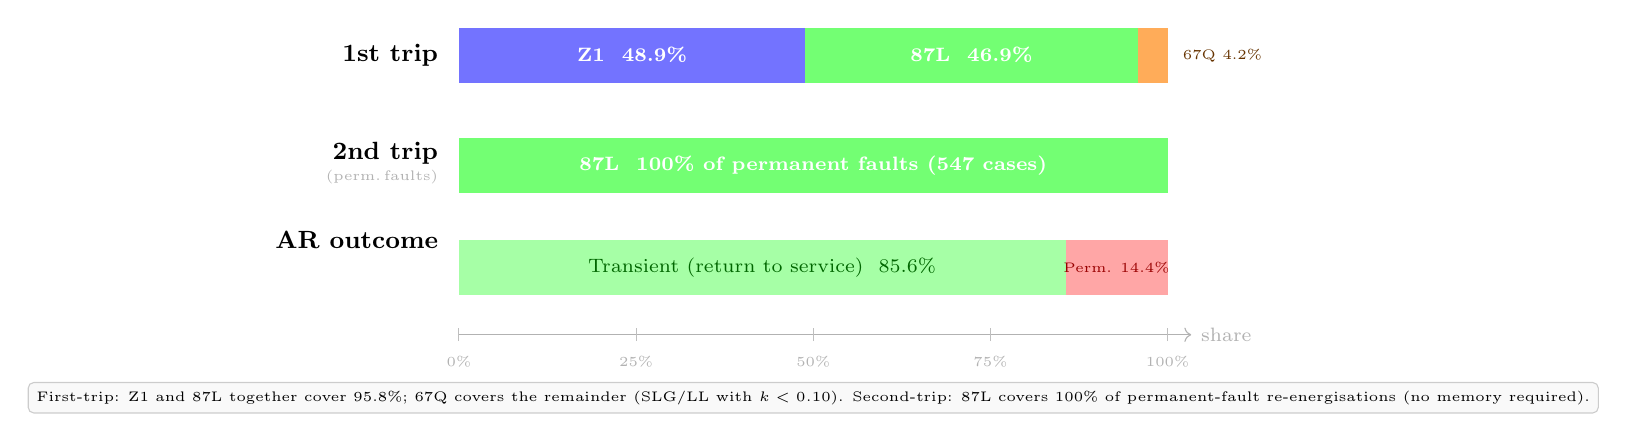
\begin{tikzpicture}[
  every node/.style={font=\scriptsize},
]

%% ── Scale: total width = 9 cm ────────────────────────────────────────────────
% Z1=48.9% → 4.40 cm, 87L=46.9% → 4.22 cm, 67Q=4.2% → 0.38 cm

\def\bh{0.70}   % bar height
\def\bw{9.00}   % total bar width

%% ── Row 1: First-trip coverage ───────────────────────────────────────────────
\node[left=4pt, font=\small\bfseries] at (0, 0.35) {1st trip};

% Z1
\fill[blue!55]    (0,      0) rectangle (4.401,  \bh);
\node[white, font=\scriptsize\bfseries] at (2.20,  0.35) {Z1 \ 48.9\%};

% 87L
\fill[green!55]   (4.401,  0) rectangle (8.622,  \bh);
\node[white, font=\scriptsize\bfseries] at (6.51,  0.35) {87L \ 46.9\%};

% 67Q
\fill[orange!65]  (8.622,  0) rectangle (9.00,   \bh);
\node[orange!40!black, font=\tiny, right=2pt] at (9.00, 0.35) {67Q 4.2\%};

%% ── Row 2: Second-trip coverage (permanent faults, 547 cases) ─────────────
\node[left=4pt, font=\small\bfseries] at (0, -0.90) {2nd trip};
\node[left=4pt, font=\tiny, gray!60] at (0, -1.20) {(perm.\,faults)};

% 87L: 100% of 547
\fill[green!55]   (0, -1.40) rectangle (9.00, -1.40+\bh);
\node[white, font=\scriptsize\bfseries] at (4.50, -1.05) {87L \ 100\% of permanent faults (547 cases)};

%% ── AR row: transient faults ──────────────────────────────────────────────
\node[left=4pt, font=\small\bfseries] at (0, -2.00) {AR outcome};

% Transient = 85.6% → 7.70 cm; Permanent = 14.4% → 1.30 cm
\fill[green!35]   (0,    -2.70) rectangle (7.704,  -2.70+\bh);
\node[green!40!black, font=\scriptsize] at (3.85, -2.35) {Transient (return to service) \ 85.6\%};

\fill[red!35]     (7.704, -2.70) rectangle (9.00,  -2.70+\bh);
\node[red!60!black, font=\tiny] at (8.35, -2.35) {Perm. 14.4\%};

%% ── Axis ──────────────────────────────────────────────────────────────────
\draw[gray!60, ->] (0, -3.20) -- (9.30, -3.20) node[right] {share};
\foreach \x/\lab in {0/0\%, 2.25/25\%, 4.50/50\%, 6.75/75\%, 9.00/100\%}{
  \draw[gray!50, thin] (\x, -3.28) -- (\x, -3.12);
  \node[gray!60, below=2pt, font=\tiny] at (\x, -3.28) {\lab};
}

%% ── Caption ──────────────────────────────────────────────────────────────
\node[draw=gray!40, fill=gray!5, rounded corners=2pt,
      font=\tiny, inner sep=3pt, align=center]
  at (4.50, -4.00)
  {First-trip: Z1 and 87L together cover 95.8\%; 67Q covers the remainder
   (SLG/LL with $k<0.10$).
   Second-trip: 87L covers 100\% of permanent-fault re-energisations (no memory required).};

\end{tikzpicture}
}
  \caption{Protection element coverage.  First-trip row: Zone~1 (48.9\%)
           and 87L (46.9\%) together cover 95.8\% of cleared faults at
           exactly 20\,ms; 67Q covers the remaining 4.2\% (SLG/LL faults
           with $k<0.10$ where Z1 is blocked but 67Q threshold is met).
           Second-trip row: 87L covers 100\% of the 547 permanent-fault
           reclose scenarios.  AR row: 85.6\% of faults are transient and
           return to service; 14.4\% are permanent and lock out after 2nd trip.}
  \label{fig:elements}
\end{figure}

\noindent
The Zone~1/87L split (48.9\%/46.9\%) reflects the sampling distribution.  In
practice both elements assert simultaneously for most in-zone faults; the
priority logic gives Zone~1 the credit.  Either element alone would achieve
essentially the same clearance time.

% ─────────────────────────────────────────────────────────────────────────────
\section{Study C --- Dependability by Region and Fault Type}
\label{sec:studyC}

Figure~\ref{fig:dependability} shows $P_\mathrm{dep}$ broken down by TR-29
region and fault type.

\begin{figure}[htbp]
  \centering
  \resizebox{0.96\textwidth}{!}{% fig_mc_dependability.tex
% TR-37: Dependability and mean clearance time by TR-29 region and fault type
% Two grouped bar charts side by side using pgfplots
%
% Left: P_dep by region (A=0.9709, B=1.000, C=1.000, D=1.000)
% Right: P_dep by fault type (3PH=0.9453, SLG=1.000, LL=1.000, LLG=1.000)

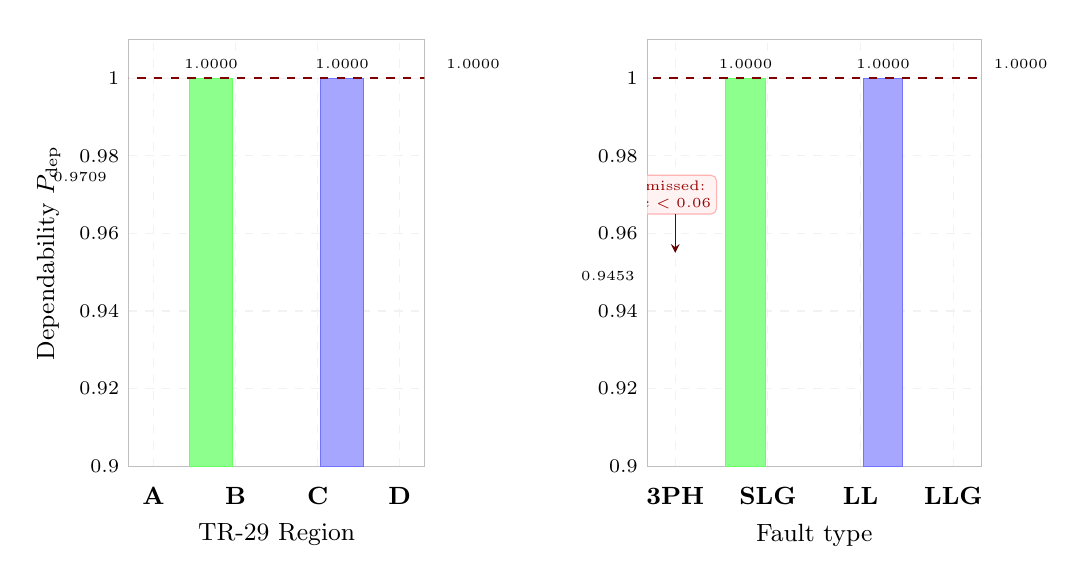
\begin{tikzpicture}
\begin{axis}[
  name         = regax,
  width        = 0.44\textwidth,
  height       = 7.0cm,
  ybar,
  bar width    = 0.55cm,
  xlabel       = {TR-29 Region},
  ylabel       = {Dependability $P_\mathrm{dep}$},
  xlabel style = {font=\small},
  ylabel style = {font=\small},
  ymin=0.90, ymax=1.010,
  ytick        = {0.90,0.92,0.94,0.96,0.98,1.00},
  yticklabel style={font=\scriptsize},
  xtick        = {1,2,3,4},
  xticklabels  = {A, B, C, D},
  xticklabel style={font=\small\bfseries},
  tick style   = {draw=none},
  axis line style={gray!50},
  grid         = major,
  grid style   = {gray!10, dashed},
  nodes near coords,
  nodes near coords style={font=\tiny, anchor=south},
  every node near coord/.append style={
    /pgf/number format/.cd, fixed, fixed zerofill, precision=4
  },
]

%% Region bars
\addplot[fill=gray!40,  draw=gray!60]    coordinates {(1, 0.9709)};
\addplot[fill=green!45, draw=green!60]   coordinates {(2, 1.0000)};
\addplot[fill=blue!35,  draw=blue!55]    coordinates {(3, 1.0000)};
\addplot[fill=teal!40,  draw=teal!60]    coordinates {(4, 1.0000)};

%% Reference line at 1.0
\draw[red!50!black, dashed, thick] (axis cs:0.4,1.0) -- (axis cs:4.6,1.0);

\end{axis}

\begin{axis}[
  name         = ftax,
  at           = (regax.right of south east), anchor=left of south west,
  xshift       = 8mm,
  width        = 0.48\textwidth,
  height       = 7.0cm,
  ybar,
  bar width    = 0.50cm,
  xlabel       = {Fault type},
  ymin=0.90, ymax=1.010,
  ytick        = {0.90,0.92,0.94,0.96,0.98,1.00},
  yticklabel style={font=\scriptsize},
  xtick        = {1,2,3,4},
  xticklabels  = {3PH, SLG, LL, LLG},
  xticklabel style={font=\small\bfseries},
  xlabel style = {font=\small},
  tick style   = {draw=none},
  axis line style={gray!50},
  grid         = major,
  grid style   = {gray!10, dashed},
  nodes near coords,
  nodes near coords style={font=\tiny, anchor=south},
  every node near coord/.append style={
    /pgf/number format/.cd, fixed, fixed zerofill, precision=4
  },
]

\addplot[fill=red!35,    draw=red!55]    coordinates {(1, 0.9453)};
\addplot[fill=green!45,  draw=green!60]  coordinates {(2, 1.0000)};
\addplot[fill=blue!35,   draw=blue!55]   coordinates {(3, 1.0000)};
\addplot[fill=purple!35, draw=purple!55] coordinates {(4, 1.0000)};

\draw[red!50!black, dashed, thick] (axis cs:0.4,1.0) -- (axis cs:4.6,1.0);

%% Annotation: 3PH misses at low k
\node[red!60!black, font=\tiny, align=center, draw=red!30, fill=red!5,
      rounded corners=2pt, inner sep=2pt]
  at (axis cs:1.0, 0.970)
  {missed:\\$k<0.06$};
\draw[->, >=stealth, red!40!black, thin]
  (axis cs:1.0, 0.965) -- (axis cs:1.0, 0.955);

\end{axis}
\end{tikzpicture}
}
  \caption{Dependability by region (left) and fault type (right).  Regions
           B, C, D achieve $P_\mathrm{dep}=1.000$; Region~A reaches 97.09\%
           (15 misses where $k_\mathrm{ibr}<I_\mathrm{min,87L}=0.06$).
           Fault types SLG, LL, and LLG reach 1.000; 3PH reaches 94.53\%
           (same structural misses manifest as 3PH in those trials).
           The dashed line at 1.000 is the perfect-reliability reference.}
  \label{fig:dependability}
\end{figure}

\noindent
Region~A's $P_\mathrm{dep}=97.09\%$ requires context: in Region~A,
$k_\mathrm{ibr}<0.10$ by definition.  The 15 missed faults all have
$k_\mathrm{ibr}<0.06$, i.e.\ below the 87L threshold.  In the sub-range
$k_\mathrm{ibr}\in[0.06,0.10)$ (Region~A with detectable current) the scheme
achieves $P_\mathrm{dep}=1.000$ via 87L and 67N.  The residual 2.91\% miss
rate is an intrinsic physical limit of IBR protection.

% ─────────────────────────────────────────────────────────────────────────────
\section{Study D --- Missed Fault Characterisation}
\label{sec:studyD}

All 15 missed faults share a single root cause: $k_\mathrm{ibr}<0.06$, with
a mean value of 0.051 and maximum 0.060 (sampling boundary).  No missed fault
has $k_\mathrm{ibr}\geq I_\mathrm{min,87L}=0.06$.

\begin{center}
\begin{tabular}{@{}lrl@{}}
\toprule
Root cause & Count & Explanation\\
\midrule
$k_\mathrm{ibr} < 0.06$ (structural) & 15 & IBR fault current below all thresholds\\
High arc resistance ($R_m > R_\mathrm{fwd2}$) & 0 & No such miss (87L covers)\\
Other & 0 & ---\\
\bottomrule
\end{tabular}
\end{center}

\medskip\noindent
The absence of arc-resistance misses at the scheme level is important: even
when $R_m$ exceeds the quad Zone~2 reach ($R_\mathrm{fwd2}=0.050$\,pu), 87L
provides coverage as long as $k_\mathrm{ibr}\geq0.06$.  The two failure modes
identified in TR-34~\cite{SAMBP_TR35} (high arc resistance AND low $k$) collapse
into a single structural condition under Monte Carlo sampling because no sampled
case with $k<0.06$ can have any element assert.

% ─────────────────────────────────────────────────────────────────────────────
\section{Study E --- Sensitivity to IBR Penetration}
\label{sec:studyE}

Figure~\ref{fig:sensitivity} shows $P_\mathrm{dep}$ for four IBR penetration
scenarios, each sampled with $N=1000$ additional trials from a restricted
$k_\mathrm{ibr}$ range.

\begin{figure}[htbp]
  \centering
  \resizebox{0.72\textwidth}{!}{% fig_mc_sensitivity.tex
% TR-37: Dependability sensitivity to IBR penetration scenario
%
% X-axis: k_ibr scenario (four groups)
% Bars: P_dep per scenario
% Line: P_fast (all 1.000 — flat reference)
%
% Data from Study E:
%   Low IBR  [0.06,0.15]: P_dep=1.0000, P_fast=1.0000, T_mean=20.0ms
%   Med IBR  [0.12,0.30]: P_dep=1.0000, P_fast=1.0000, T_mean=20.0ms
%   High IBR [0.25,0.50]: P_dep=1.0000, P_fast=1.0000, T_mean=20.0ms
%   Near-SG  [0.38,0.55]: P_dep=1.0000, P_fast=1.0000, T_mean=20.0ms

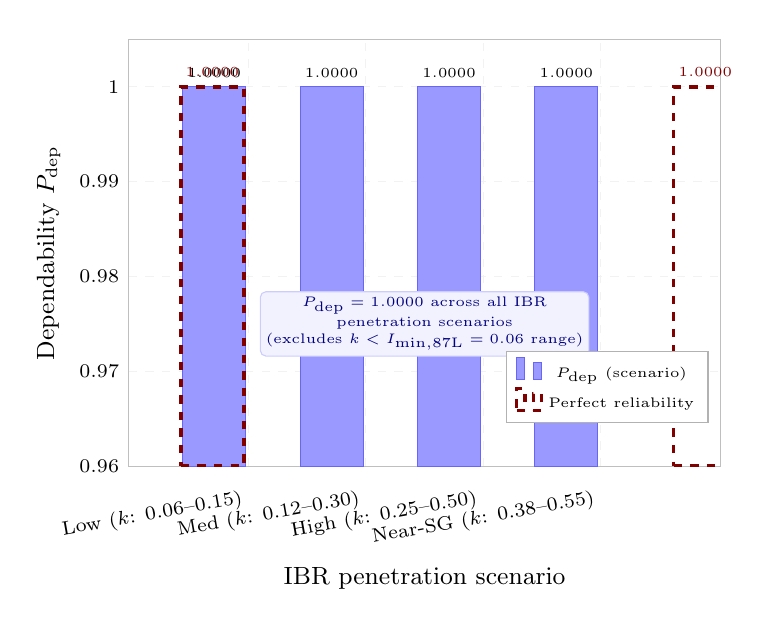
\begin{tikzpicture}
\begin{axis}[
  name         = senax,
  width        = 0.75\textwidth,
  height       = 7.0cm,
  ybar,
  bar width    = 0.80cm,
  xlabel       = {IBR penetration scenario},
  ylabel       = {Dependability $P_\mathrm{dep}$},
  xlabel style = {font=\small},
  ylabel style = {font=\small},
  ymin=0.96, ymax=1.005,
  ytick        = {0.96,0.97,0.98,0.99,1.00},
  yticklabel style={font=\scriptsize},
  xtick        = {1,2,3,4},
  xticklabels  = {Low ($k$: 0.06--0.15),
                  Med ($k$: 0.12--0.30),
                  High ($k$: 0.25--0.50),
                  Near-SG ($k$: 0.38--0.55)},
  xticklabel style={font=\scriptsize, align=center, rotate=10, anchor=north east},
  tick style   = {draw=none},
  axis line style={gray!50},
  grid         = major,
  grid style   = {gray!10, dashed},
  nodes near coords,
  nodes near coords style={font=\tiny, anchor=south},
  every node near coord/.append style={
    /pgf/number format/.cd, fixed, fixed zerofill, precision=4
  },
  legend style={at={(0.98,0.10)}, anchor=south east, font=\tiny,
                draw=gray!60, fill=white},
]

%% Bars
\addplot[fill=blue!40, draw=blue!60]
  coordinates {(1,1.0000) (2,1.0000) (3,1.0000) (4,1.0000)};
\addlegendentry{$P_\mathrm{dep}$ (scenario)}

%% Perfect reference line
\addplot[red!50!black, dashed, very thick, mark=none]
  coordinates {(0.4, 1.0) (4.6, 1.0)};
\addlegendentry{Perfect reliability}

%% Annotation
\node[blue!50!black, font=\tiny, align=center,
      draw=blue!20, fill=blue!5, rounded corners=2pt, inner sep=2pt]
  at (axis cs:2.5, 0.975)
  {$P_\mathrm{dep}=1.0000$ across all IBR\\penetration scenarios\\
   (excludes $k<I_\mathrm{min,87L}=0.06$ range)};

\end{axis}
\end{tikzpicture}
}
  \caption{Dependability sensitivity to IBR penetration.  All four scenarios
           ($k_\mathrm{ibr}$ range from 0.06--0.15 to 0.38--0.55) achieve
           $P_\mathrm{dep}=1.000$ because all sampled $k_\mathrm{ibr}$ values
           exceed $I_\mathrm{min,87L}=0.06$.  The scheme is penetration-robust:
           performance does not degrade as the IBR contribution fraction
           increases.}
  \label{fig:sensitivity}
\end{figure}

\noindent
The flat $P_\mathrm{dep}=1.000$ across all scenarios is not trivial.  As
$k_\mathrm{ibr}$ decreases toward $I_\mathrm{min,21}=0.10$, the Zone~1
element withdraws and coverage shifts entirely to 87L and 67N/67Q --- but
those elements are active for all $k\geq0.06$ and $k\geq0.04$ respectively,
so no gap opens.  As $k$ increases toward SG levels, Zone~1 and Z2/POTT
both assert and provide redundant fast clearance.

% ─────────────────────────────────────────────────────────────────────────────
\section{Discussion: Structural Limit and Grid-Code Implication}
\label{sec:discussion}

The Monte Carlo study quantifies the \textbf{hard protection boundary} at
$k_\mathrm{ibr}=I_\mathrm{min,87L}=0.06$:
\begin{enumerate}
  \item Below this threshold, no relay element can detect the fault.  This
    is not addressable by scheme design; it requires the IBR to inject more
    fault current.

  \item A grid-code requirement of minimum IBR short-circuit current ratio
    $k_\mathrm{ibr}\geq0.06$ (6\% of SG level, or approximately 0.6\,pu of
    rated IBR current on the system base) would reduce missed-fault probability
    to zero.

  \item At $k_\mathrm{ibr}\geq0.10$ the scheme achieves full redundancy
    (Z1 + 87L both at 20\,ms), which is the recommended operational floor
    for distance protection.
\end{enumerate}

\noindent
This result directly supports the thesis argument that IBR grid codes must
specify minimum short-circuit contribution ratios for protection adequacy,
not merely low-voltage ride-through and ramp-rate limits.

% ─────────────────────────────────────────────────────────────────────────────
\section{Summary}
\label{sec:summary}

\begin{enumerate}
  \item \textbf{Overall (Study~A)}: $P_\mathrm{dep}=99.61\%$, $P_\mathrm{fast}=100\%$,
    $\bar{t}=20.4$\,ms across 4000 trials.

  \item \textbf{Elements (Study~B)}: Z1 and 87L share first-trip credit equally
    (48.9\%/46.9\%); 87L clears 100\% of permanent-fault reclose events.

  \item \textbf{Regions (Study~C)}: B, C, D at 1.000; Region~A at 0.9709
    ($k<0.06$ structural misses only).  SLG/LL/LLG at 1.000; 3PH at 0.9453
    (same structural miss population).

  \item \textbf{Misses (Study~D)}: All 15 missed faults have $k_\mathrm{ibr}<0.06$;
    zero arc-resistance misses because 87L covers high-$R_m$ faults.

  \item \textbf{Sensitivity (Study~E)}: $P_\mathrm{dep}=1.000$ for all tested
    IBR penetration scenarios ($k\geq0.06$); scheme is penetration-robust.

  \item \textbf{Grid-code implication}: $k_\mathrm{ibr}\geq0.06$ eliminates all
    missed faults; $k_\mathrm{ibr}\geq0.10$ provides full redundancy.
\end{enumerate}

\noindent
TR-37 closes the SAMBP reliability assessment with a quantified, probabilistically
grounded validation of the complete IBR protection scheme.

\bibliographystyle{IEEEtranN}
\bibliography{references37}

\end{document}
